\section{Assignment 2: Image Segmentation by $K-$means\ \ Clustering}
\label{sec:assignment2}

In this assignment we use K-means clustering for image segmentation. K-means clustering is a very simple but effective clustering algorithm, but it also comes with some drawbacks. We examine the strengths and weaknesses of this method applied to image segmentation.

\subsection{Problem definition}

Given an image, the goal is to divide it into disjoint regions. These regions should correspond to coherent areas in the image. In  a perfect result, each ``object'' is matched to exactly one region. What an ``object'' is, depends on the application: we might want to separate different colors or textures, or to separate the background from the foreground, or obtain a region for each physical object in the image. In this assignment we examine K-means clustering applied to image segmentation.
 In particular we:
\begin{itemize}[noitemsep]
	\item Implement K-means clustering.
	\item Study the influence of augmenting the color information with spatial information in the form of normalized pixel coordinates.
	\item Study the influence of the number of clusters chosen.
	\item Discuss the advantages and disadvantages of K-means clustering for image segmentation.
\end{itemize}

\subsection{Methodology}

\subsubsection{Overview}
K-means clustering is an algorithm used to cluster data. It works as follows: assume we have data $x_1,\ldots,x_N \in \mathbb{R}^n$. We first chose K centroids $\mu_k \in \mathbb{R}^n$ randomly. Then we assign each data point $x_i$ to the centroid $\mu_j$ which minimizes the distance between $x_i$ and the centroids $\mu_k$. To record this relation we use an indicator matrix $r(i,j) \in \{0,1\}$, with $r(i,j)=1$ if data point $x_i$ is assigned to centroid $\mu_j$ and $0$ otherwise. We can define an objective function, which the K-means clustering algorithm tries to minimize. For this we define the distortion as
\begin{equation}
	J = \sum_{n=1}^{N} \sum_{k=1}^{K} r(n,k) \left\|x_n-\mu_k\right\|^2.
\end{equation}
This is the sum of squared distances from each data point to its assigned centroid, and we want to minimize it. For this we use the following iterative K-means clustering method:
\begin{enumerate}
\item Initialize the $K$ centroids $\mu_k$ with random values.
\item Assign each data point $x_i$ to its nearest centroid $\mu_j$ and update the indicator matrix
\[
	r(i,j)= \begin{cases}
               1 \text{, if } j = \argmin_k\left\|x_i-\mu_k\right\| \\

             0 \text{ otherwise.}
            \end{cases}
\]
\item Calculate new centroids $\mu_k$ as the mean of all data points assigned to the k-th cluster, i.e. 
\[
	\mu_k = \frac{\sum\limits_{i=1}^N r(i,k) x_i}{\sum\limits_{i=1}^N r(i,k)}
\]
\item Calculate the distortion J with the new assignment and centroids and check for convergence. This is done by checking if the ratio of the old and new $J$ does not change any more, i.e if the ratio lies below a user given threshold. We use the absolute value of 1 minus the ratio, so that the algorithm can also make $J$ a little worse, as this could make the end result better. As long as J does not converge, repeat steps 2 to 4.
\end{enumerate} 

We use two different methods to get data points from pixel values. One is to just take the color values of each pixel, the other is to normalize each coordinate of a pixel to $[0, 1]$ and use the color value and the coordinate of the pixel, resulting in a 5-dimensional space.

To illustrate the results we can color each pixel in the image with the color of the associated centroid. Alternatively we can associate the clusters with mutually distinct colors and colorize the image using these, instead of the value of the centre. This helps to better see the cluster boundaries.

\subsubsection{Implementation}

The image segmentation can be run with the function \texttt{image\_segmentation(image\_path, K, precision, use\_coordinates, use\_distinct\_colors)}, where \texttt{image\_path} is the path to the image, \texttt{K} is number of clusters, \texttt{precision} is the precision used for the convergence criterion of the distortion, \texttt{use\_coordinates} is a boolean that determines if coordinates should be used or not, and \texttt{use\_distinctcolors} is another boolean, deciding if the result shall be colorized with distinct colors (if true) or by using the color of the cluster center (if false). It returns the segmented image, colored with the chosen option, the cluster centroids and the indicator matrix.
 We explain some details of the implementation below.

To make use of vectorization and matrix operations we vectorize the image. That means that instead of indexing pixels by two indexes we use just one. This has the advantage that the indicator matrix is a two dimensional matrix. Thus, $r(i,j)*\text{centroids}$ (where centroids is the vector of centroids) evaluates to the centroid associated with each data point. And if $X$ is the data matrix, i.e $X(i,:)$ is the i-th data point, then $r(i,j)^T * X$ equals the sum of all data points associated with one cluster.

As mentioned above we use $\vert 1-J_{old}/J_{new}\vert < \text{precision}$ as a convergence criterion, where we take absolute values to allow the objective value to also get worse in the hope of not getting stuck in a local minimum.

One problem is that calculating the mean of the data of a cluster is not possible, if the cluster is empty. This can happen in the assignment stage. To fix this, for each empty cluster we choose a random data point, remove it from its original cluster and add it to the empty cluster.

The function distinguishable\_colors was taken from mathworks.com/matlabcentral/fileexchange and the relevant license is included.
\subsection{Experiments}

We analyzed K-means clustering for image segmentation with the test images \texttt{future.jpg}, \texttt{mm.jpg} and \texttt{simple.PNG}, and made the following experiments. First we clustered each image into 3 and 5 clusters, both with and without the use of coordinates. Then we separately examined the image \texttt{mm.jpg}. We used different K values and varied the use of coordinates. We also ran the algorithm several times on \texttt{simple.PNG} to show the effect of bad initialization.

In Figure \ref{fig:testimages} the test images are shown. \texttt{future.jpg} is a hand-drawn image, containing only a restricted color palette. Test image \texttt{mm.jpg} is a photography of an advertisement screen. It has a lot of artifacts in the screen and many fine details in the background which makes segmentation more difficult. The third test image, \texttt{simple.PNG}, is an artificially generated image. It just contains 2 filled circles on an uniform background, which makes it very easy to segment.
\begin{figure}[h!]
	
\includegraphics[width=0.38\linewidth]{figures/task2/future.jpg}
	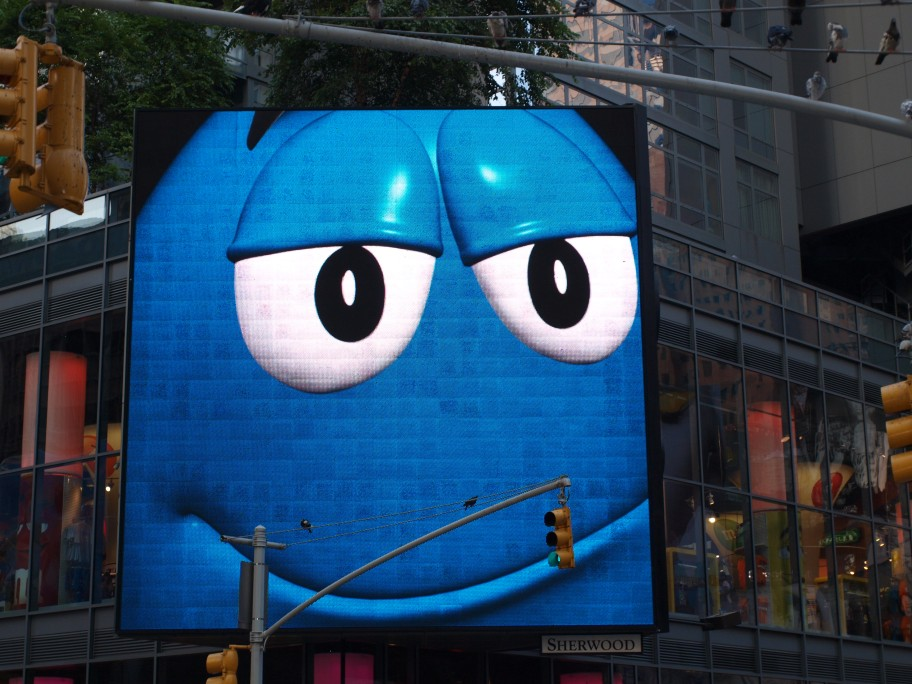
\includegraphics[width=0.398\linewidth]{figures/task2/mm.jpg}
	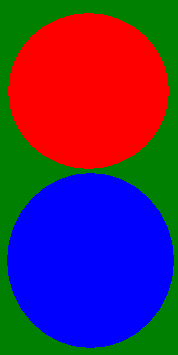
\includegraphics[width=0.15\linewidth]{figures/task2/simple.PNG}
	\caption{The 3 test images. From left to right: \texttt{future}, \texttt{mm} and \texttt{simple}.}
	\label{fig:testimages}
\end{figure}

\subsubsection{Influence of using coordinates}

Figures \ref{fig:future:coords} -- \ref{fig:simple:coords} illustrate the result of the segmentation by coloring each pixel by the color value of its associated centroid. We show the influence of the usage of coordinates for K=3 and K=5 clusters for each test image.

\begin{figure}[h!]
\centering
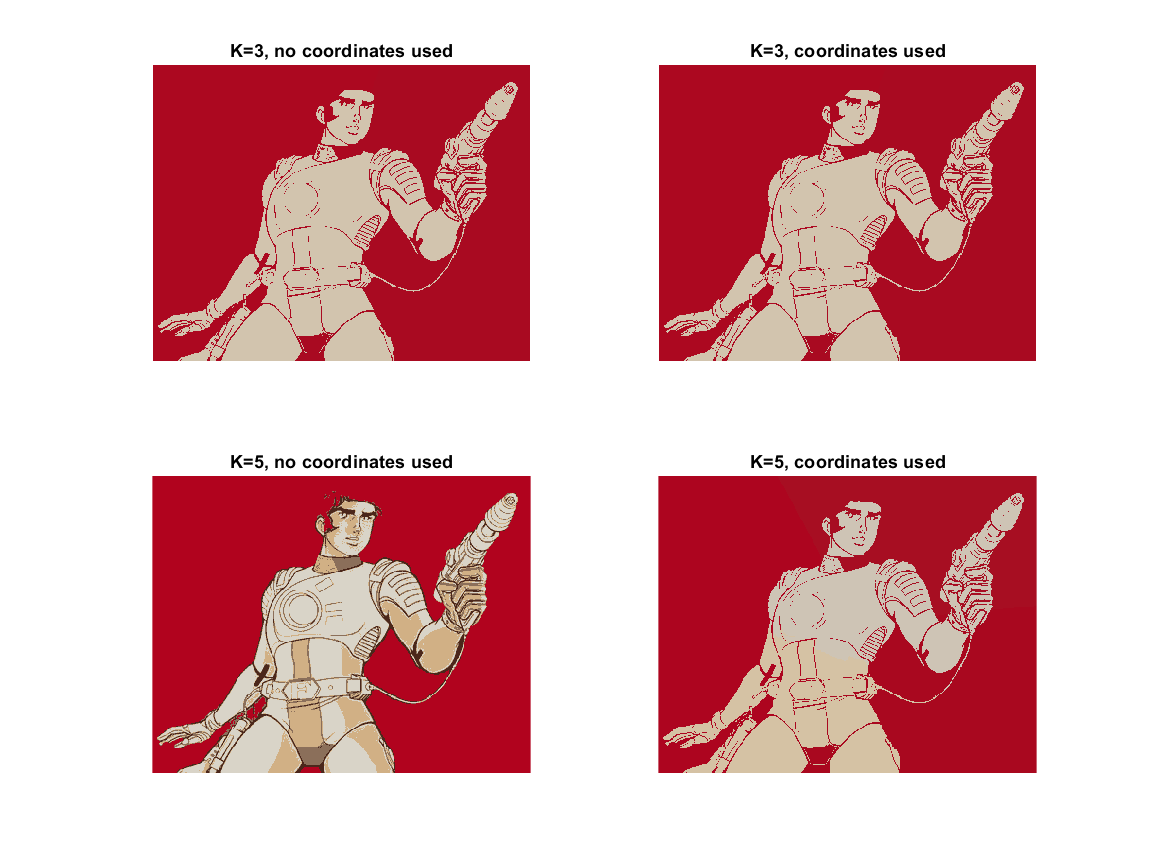
\includegraphics[width = 0.95\linewidth]{figures/task2/future_coordinates.png}
\caption{Coordinate experiment for \texttt{future.jpg}}
\label{fig:future:coords}
\end{figure}

The results for the image \texttt{future.jpg} are shown in Figure \ref{fig:future:coords}. It can be seen that the segmentation without using coordinates produces a pleasing result. It can separate the different colors very accurately. This is the case because the image contains only a limited number of colors, and all colors in a coherent region have the same color. For the clustering with coordinates it appears that the algorithm found less clusters than K. This is due to the background getting segmented into multiple regions. This happens, because the pixels on the right and on the left have the same color on one hand, but are spatially far apart, so it makes sense to split the background in a left region and right region. For $K=5$ the image gets split into 3 background regions, a top part of person region and a bottom part of person region. It can be seen that not only the color, but also the spacial relation is important. Also observable is that using the colors of the cluster center makes the inspection of the result hard, as several cluster, in particular for the case which uses coordinates, can have the same or very similar colors.

\begin{figure}[h!]
\centering
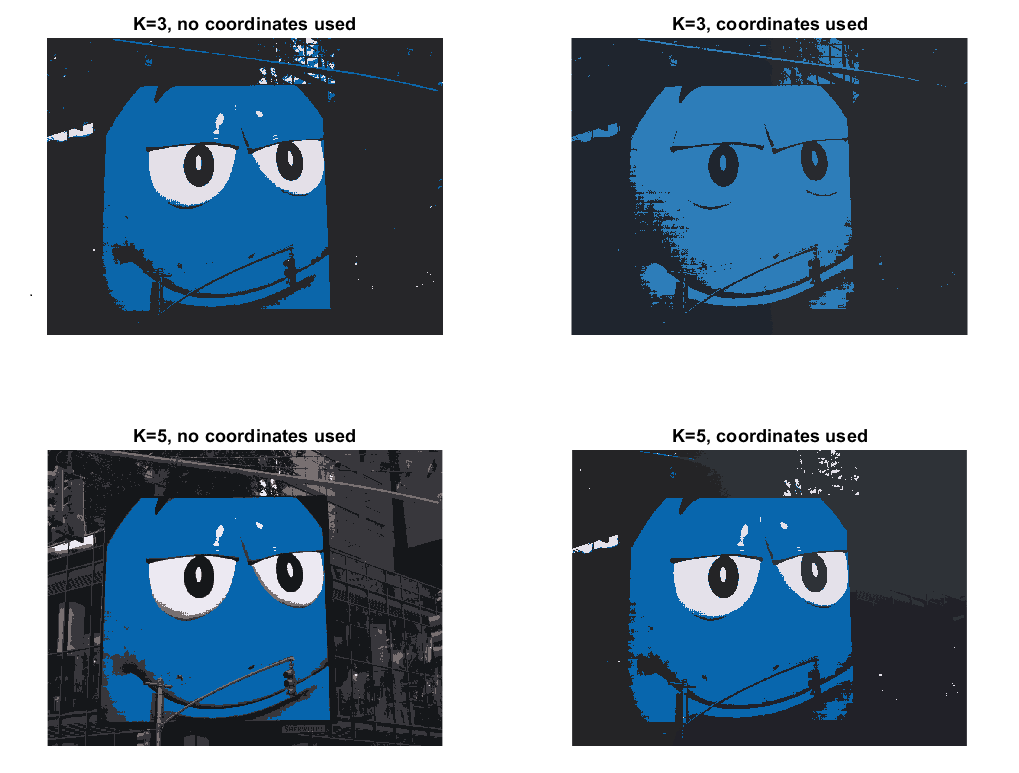
\includegraphics[width = 0.8\linewidth]{figures/task2/mm_coordinates.png}
\caption{Coordinate experiment for \texttt{mm.jpg}}
\label{fig:mm:coords}
\end{figure}

The results for the image \texttt{mm.jpg}, shown in Figure \ref{fig:mm:coords}, are hard to interpret, because one can not well distinguish the different clusters, as they have very similar colors (this is discussed below). Therefore we repeated the experiment for $K=5$ and used distinct colors. The result is shown in Figure \ref{fig:mm:coords:distinct}. 

For $K=3$ without coordinates, the image gets separated into a white, black and blue region. With the use of coordinates, it again is separated into a blue foreground region and 2 background regions. As the average of the background is similar everywhere, the different clusters can not be seen. For K=5, the image gets separated into 5 colors. As only the color is important, a lot of fine details are visible in the background; on the other hand, if we use coordinates, those fine details are not preserved, as they do not form a connected region. K-means basically produces a Voronoi tessellation of the space. Therefore the regions should be polygons or circles. If distinct colors are used, Figure \ref{fig:mm:coords:distinct} clearly demonstrates that only using colors produces very irregular structures spatially-wise, as they are only defined by color and not their spacial relation. On the other hand, if we use coordinates the algorithm produces regular spatial regions; irregularities only occur on the border between two regions, as at that position color is more important, because the distance in the spatial domain to the two centres is equal.

\begin{figure}[h!]
\centering
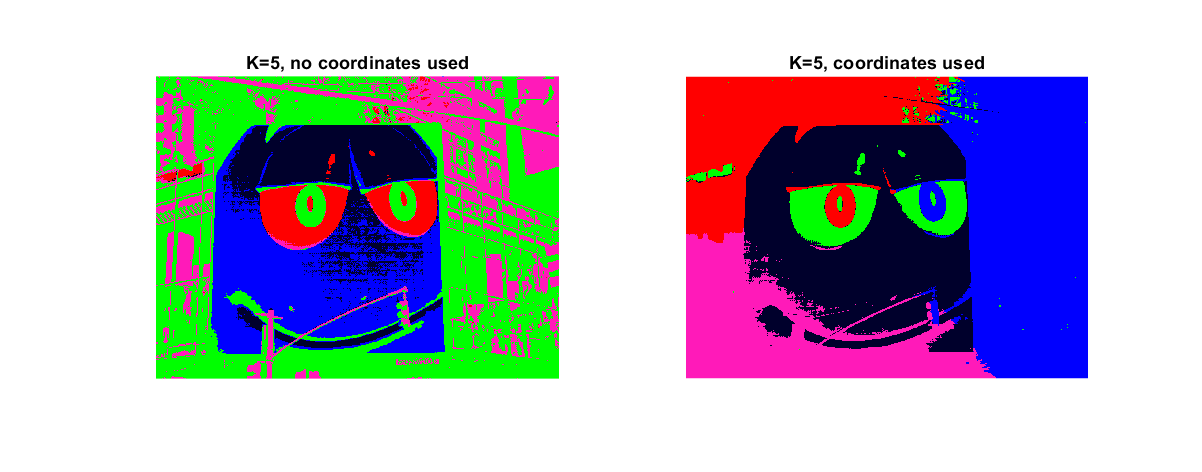
\includegraphics[width = 0.9\linewidth]{figures/task2/mm_bad_visibility.png}
\caption{Coordinate experiment for \texttt{mm.jpg} with distinct colors.}
\label{fig:mm:coords:distinct}
\end{figure}

The clustering algorithm has no problem segmenting an image like \texttt{simple.PNG}. For $K=5$ the algorithm has to produce too many clusters. Without spatial information it just creates two extra clusters containing only a single pixel. With spatial information, it divides two of the cluster into a left and right part, or top and bottom part.

\begin{figure}[h!]
\centering
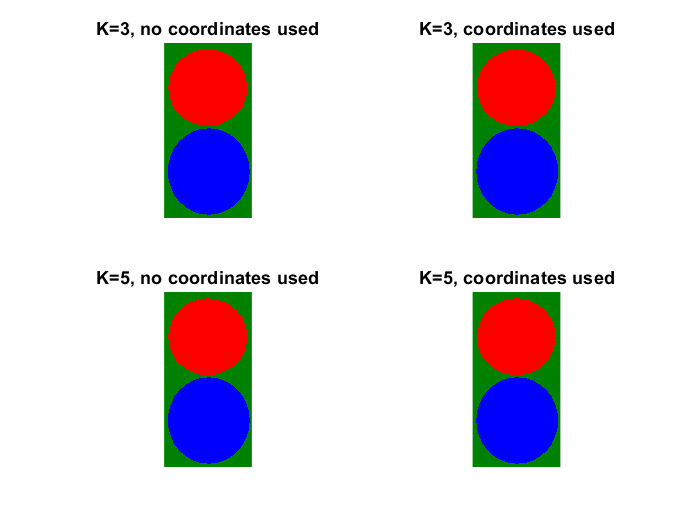
\includegraphics[width = 0.7\linewidth]{figures/task2/simple_coordinates.png}
\caption{Coordinate experiment for \texttt{simple.PNG}}
\label{fig:simple:coords}
\end{figure}

\subsubsection{Experimenting with the number of clusters}
In a second experiment we took the picture \texttt{mm.jpg} and segmented it using different number of clusters, again both with and without using coordinates. The results are shown in Figure \ref{fig:mm:nocoords:manyK} and \ref{fig:mm:coords:manyK}. We used distinct colors for colorization, in order to better distinguish the resulting clusters.

\begin{figure}[h!]
\centering
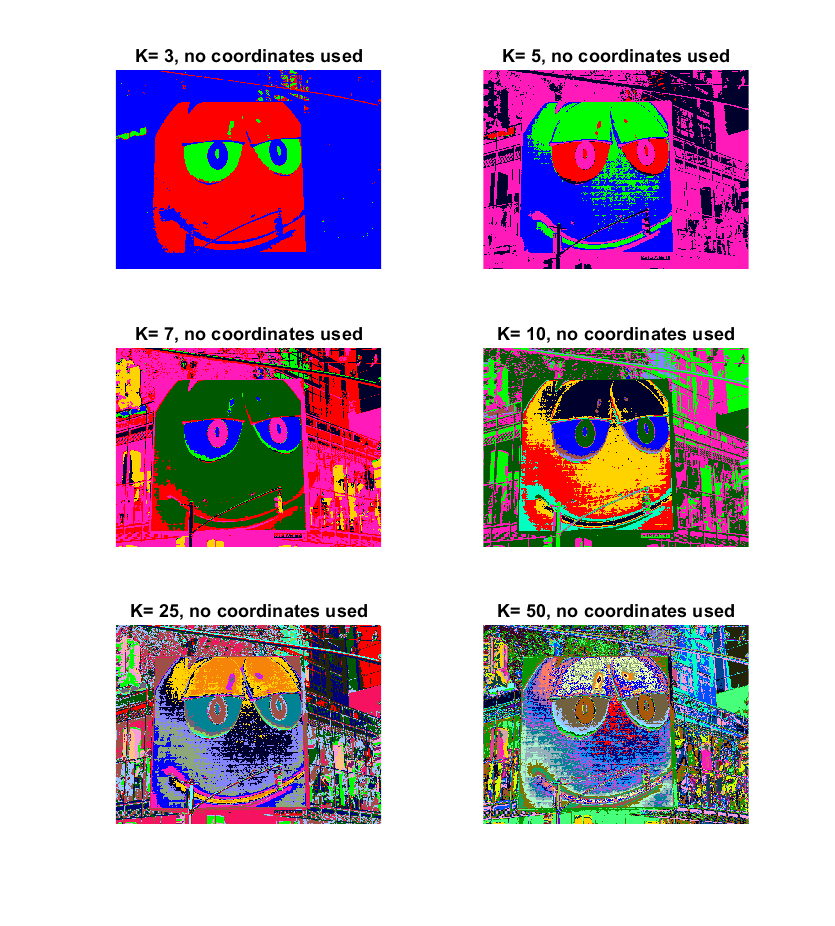
\includegraphics[width =0.8\linewidth]{figures/task2/mm_nocoords_manyK.png}
\caption{Clustering with different values of K without use of coordinates}
\label{fig:mm:nocoords:manyK}
\end{figure}

Different trends can be observed. First, it can be seen that without coordinates the clusters get more and more irregular. The higher the number of clusters, the less a cluster corresponds to a physical object. This is because an object consists of many, although similar, colors and as the spatial relation is missing, the algorithm can not know which regions belong together. If we color the image with the cluster centroids, the result is visually similar to the original picture; this could be used for image compression. It can also be seen, that for a relatively low number of clusters the fine details in the background, like windows or the scaffolding, are preserved, but for higher numbers such details disappear and the clusters more closely resemble noise.

\begin{figure}[h!]
\centering
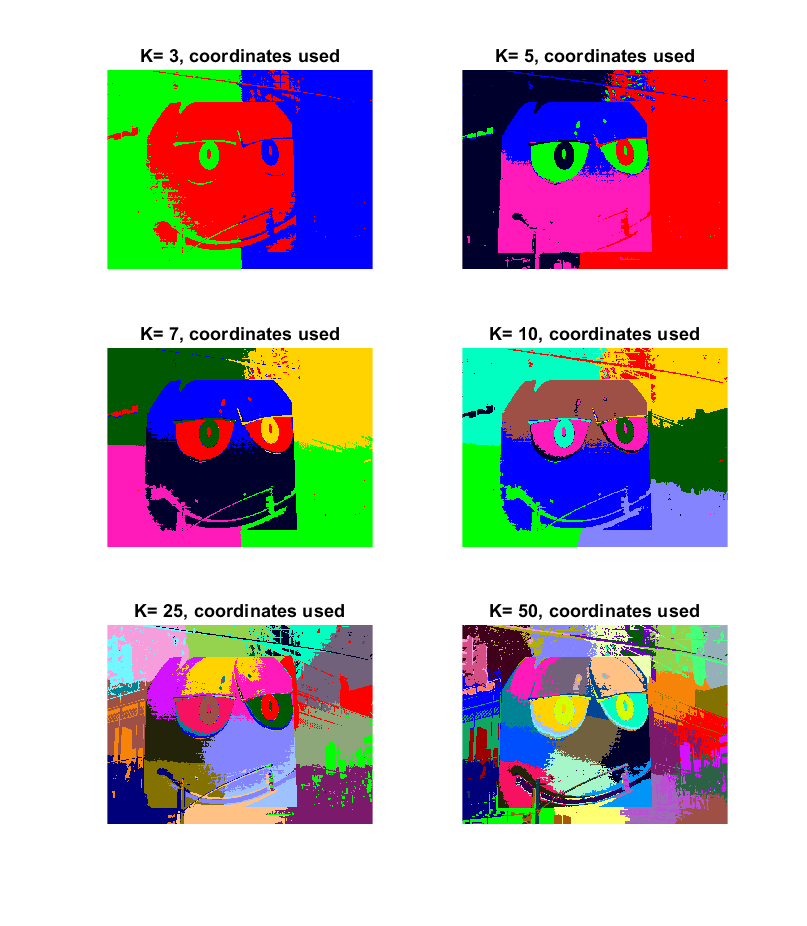
\includegraphics[width =0.8\linewidth]{figures/task2/mm_coords_manyK.png}
\caption{Clustering with different values of K without use of coordinates}
\label{fig:mm:coords:manyK}
\end{figure}

For the case with coordinates, as shown in Figure \ref{fig:mm:coords:manyK}, the algorithm tends to produce spatially connected regions. Also the splitting of the regions into multiple clusters, as the number of clusters increases, is visible, as mentioned above. We observed that the coordinates force the regions to become more like closed polygons. This makes it impossible to segment spatially irregular structures like the scaffolding and windows, even if requesting a very large number of clusters. 

\section{Discussion}
Immediately obvious is, that the main strength of the K-means clustering algorithm is that it uses no domain knowledge. This general algorithm could be taken as-is and applied to image segmentation, producing somewhat useful results. So it can be very useful to use K-means clustering as a baseline method to compare other methods against. It is also a very simple algorithm and we can just use more features if we wish to have a more accurate result, where ``accurate'' depends on the application of course.

We also saw in our experiments that the benefit of using coordinate information or not depends mostly on the application. If we want to compress an image by using only a handful of colors, using just color information is much better. Also if we are interested in non polygonal structures, not using coordinates can lead to better results. But if we have a large number of clusters and do not use coordinates the different clusters correspond less and less to semantically coherent regions. If we use coordinates, we get spatially connected regions. This can be useful in some applications. Imaginable would be, for instance, to post-process an image which was segmented with K-means clustering using many clusters by merging clusters that are very similar, based on some metric. This metric could use other features.

One main disadvantage is that the result can vary a lot with different initializations, as demonstrated in Figure \ref{fig:simple:badinit}. We can circumvent this by using a deterministic initialization. Moreover for every pixel the distance to every cluster has to be calculated. This can be computationally expensive for large images or large number of clusters. Moreover there is no guarantee that the distortion does not end up in a local minimum. And, as the results strongly depends on the initialization, we get a different result each time we run the algorithm. This could be bad as we can not know which clusters corresponds to which part of the image, without looking at the result. This makes the performance of the algorithm unpredictable.

\begin{figure}[h!]
\centering
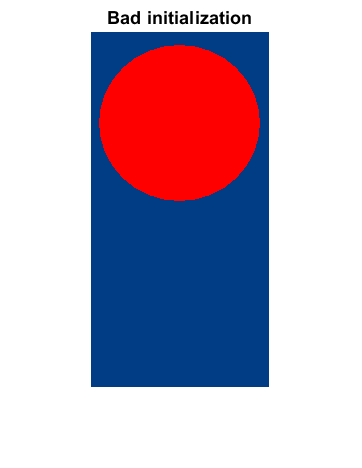
\includegraphics[width =0.5\linewidth]{figures/task2/bad_initialization.png}
\caption{Clustering with different values of K without use of coordinates}
\label{fig:simple:badinit}
\end{figure}